\documentclass[11pt]{article}

\usepackage[a4paper,margin=1in]{geometry}
\usepackage{amsmath,amssymb,amsthm,mathtools}
\usepackage{enumitem}
\usepackage{hyperref}

%\usepackage{booktabs}
%\usepackage{pgfplots}
%\pgfplotsset{compat=1.18}

\usepackage{booktabs}
\usepackage{array}
\usepackage{xcolor}
\usepackage{pgfplots}
\pgfplotsset{compat=1.18}

\hypersetup{
	colorlinks=true,
	linkcolor=blue,
	urlcolor=blue,
	citecolor=blue
}

\newcommand{\F}{\mathbb{F}}
\newcommand{\GL}{\operatorname{GL}}
\newcommand{\Mat}{\operatorname{Mat}}
\newcommand{\Span}{\operatorname{span}}
\newcommand{\Ker}{\operatorname{Ker}}
\newcommand{\im}{\operatorname{Im}}
\newcommand{\rank}{\operatorname{rank}}
\newcommand{\Prob}{\mathbb{P}}

\theoremstyle{definition}
\newtheorem{definition}{Definition}[section]
\newtheorem{example}[definition]{Example}
\newtheorem{remark}[definition]{Remark}

\theoremstyle{plain}
\newtheorem{proposition}[definition]{Proposition}
\newtheorem{theorem}[definition]{Theorem}
\newtheorem{corollary}[definition]{Corollary}

\title{Lecture Notes on the Ratio \(\lvert GL_m(\F_q)\rvert / \lvert \Mat_m(\F_q)\rvert\)}
\author{}
\date{}

\begin{document}
	
	\maketitle
	
	\tableofcontents
	
	\section{Introduction}
	
	The goal of these notes is to understand the ratio
	\[
	\frac{|GL_m(\F_q)|}{|\Mat_m(\F_q)|}.
	\]
	Here:
	\begin{itemize}[leftmargin=2em]
		\item \(\F_q\) is the finite field with \(q\) elements,
		\item \(\Mat_m(\F_q)\) denotes the set of all \(m\times m\) matrices over \(\F_q\),
		\item \(GL_m(\F_q)\) denotes the set of all invertible \(m\times m\) matrices over \(\F_q\).
	\end{itemize}
	
	This ratio has a simple probabilistic meaning:
	
	\begin{quote}
		If one chooses a matrix uniformly at random from \(\Mat_m(\F_q)\), then
		\[
		\frac{|GL_m(\F_q)|}{|\Mat_m(\F_q)|}
		\]
		is exactly the probability that the matrix is invertible.
	\end{quote}
	
	So our aim is to compute this ratio explicitly and understand what it means.
	
	\section{The ambient set of all matrices}
	
	\begin{definition}
		For \(m\in \mathbb{Z}_{>0}\), let
		\[
		\Mat_m(\F_q)=\F_q^{m\times m}
		\]
		denote the set of all \(m\times m\) matrices over \(\F_q\).
	\end{definition}
	
	\begin{proposition}
		The number of \(m\times m\) matrices over \(\F_q\) is
		\[
		|\Mat_m(\F_q)|=q^{m^2}.
		\]
	\end{proposition}
	
	\begin{proof}
		An \(m\times m\) matrix has \(m^2\) entries, and each entry can be chosen independently from \(\F_q\), which has \(q\) elements. Hence the total number of such matrices is
		\[
		\underbrace{q\cdot q\cdot \dots \cdot q}_{m^2\text{ factors}}=q^{m^2}.
		\]
	\end{proof}
	
	\begin{remark}
		Thus \(\Mat_m(\F_q)\) is the full space of all linear endomorphisms \(\F_q^m\to \F_q^m\), while \(GL_m(\F_q)\) is the subset of those endomorphisms that are invertible.
	\end{remark}
	
	\section{The general linear group}
	
	\begin{definition}
		The \emph{general linear group} over \(\F_q\) is
		\[
		GL_m(\F_q)=\{A\in \Mat_m(\F_q): A \text{ is invertible}\}.
		\]
	\end{definition}
	
	\begin{remark}
		A matrix \(A\in \Mat_m(\F_q)\) is invertible if and only if the associated linear map
		\[
		T_A:\F_q^m\to \F_q^m,\qquad x\mapsto Ax
		\]
		is bijective.
	\end{remark}
	
	\section{Why invertibility is equivalent to linear independence of columns}
	
	Let
	\[
	A=
	\begin{pmatrix}
		| & | & & |\\
		v_1 & v_2 & \cdots & v_m\\
		| & | & & |
	\end{pmatrix}
	\in \Mat_m(\F_q),
	\]
	where \(v_1,\dots,v_m\in \F_q^m\) are the columns of \(A\).
	
	\begin{proposition}
		The matrix \(A\) is invertible if and only if its columns \(v_1,\dots,v_m\) are linearly independent.
	\end{proposition}
	
	\begin{proof}
		Consider the linear map
		\[
		T_A:\F_q^m\to \F_q^m,\qquad x\mapsto Ax.
		\]
		Since \(A\) is a square matrix, \(A\) is invertible if and only if \(T_A\) is bijective.
		
		Now let
		\[
		x=
		\begin{pmatrix}
			x_1\\
			\vdots\\
			x_m
		\end{pmatrix}\in \F_q^m.
		\]
		Then
		\[
		Ax=x_1v_1+\cdots+x_mv_m.
		\]
		Therefore
		\[
		Ax=0
		\quad\Longleftrightarrow\quad
		x_1v_1+\cdots+x_mv_m=0.
		\]
		So the columns \(v_1,\dots,v_m\) are linearly independent if and only if the only solution to \(Ax=0\) is \(x=0\), that is,
		\[
		\Ker(A)=\{0\}.
		\]
		Since \(A:\F_q^m\to \F_q^m\) is a linear map between vector spaces of the same dimension, \(\Ker(A)=\{0\}\) is equivalent to injectivity, and injectivity is equivalent to bijectivity. Hence \(A\) is invertible if and only if its columns are linearly independent.
	\end{proof}
	
	\section{Counting invertible matrices}
	
	\begin{theorem}
		Let \(m\in \mathbb{Z}_{>0}\). Then
		\[
		|GL_m(\F_q)|=(q^m-1)(q^m-q)(q^m-q^2)\cdots(q^m-q^{m-1}).
		\]
		Equivalently,
		\[
		|GL_m(\F_q)|=\prod_{i=0}^{m-1}(q^m-q^i).
		\]
	\end{theorem}
	
	\begin{proof}
		We count invertible matrices column by column.
		
		An \(m\times m\) matrix is invertible if and only if its columns are linearly independent.
		
		\medskip
		
		\noindent\textbf{First column.}
		The first column may be any nonzero vector in \(\F_q^m\). Since \(\F_q^m\) has \(q^m\) vectors total and exactly one of them is zero, there are
		\[
		q^m-1
		\]
		choices.
		
		\medskip
		
		\noindent\textbf{Second column.}
		Once the first column has been chosen, the second column must not lie in its span. Since the span of a nonzero vector is a \(1\)-dimensional subspace of \(\F_q^m\), it has exactly \(q\) elements. Therefore there are
		\[
		q^m-q
		\]
		choices for the second column.
		
		\medskip
		
		\noindent\textbf{Third column.}
		Once the first two columns are linearly independent, their span is a \(2\)-dimensional subspace of \(\F_q^m\), hence has exactly \(q^2\) elements. Therefore there are
		\[
		q^m-q^2
		\]
		choices for the third column.
		
		\medskip
		
		Continuing in this way, once \(i\) linearly independent columns have been chosen, their span is an \(i\)-dimensional subspace of \(\F_q^m\), so it has exactly \(q^i\) elements. Therefore the next column can be chosen in
		\[
		q^m-q^i
		\]
		ways.
		
		Multiplying all these choices gives
		\[
		|GL_m(\F_q)|=(q^m-1)(q^m-q)(q^m-q^2)\cdots(q^m-q^{m-1}).
		\]
	\end{proof}
	
	\section{The ratio \(\lvert GL_m(\F_q)\rvert / \lvert \Mat_m(\F_q)\rvert\)}
	
	Now we divide the number of invertible matrices by the number of all matrices.
	
	\begin{theorem}
		For every \(m\ge 1\),
		\[
		\frac{|GL_m(\F_q)|}{|\Mat_m(\F_q)|}
		=
		\frac{(q^m-1)(q^m-q)(q^m-q^2)\cdots(q^m-q^{m-1})}{q^{m^2}}.
		\]
		Equivalently,
		\[
		\frac{|GL_m(\F_q)|}{|\Mat_m(\F_q)|}
		=
		\prod_{j=1}^{m}(1-q^{-j}).
		\]
	\end{theorem}
	
	\begin{proof}
		From the previous sections,
		\[
		|GL_m(\F_q)|=\prod_{i=0}^{m-1}(q^m-q^i)
		\qquad\text{and}\qquad
		|\Mat_m(\F_q)|=q^{m^2}.
		\]
		Hence
		\[
		\frac{|GL_m(\F_q)|}{|\Mat_m(\F_q)|}
		=
		\frac{\prod_{i=0}^{m-1}(q^m-q^i)}{q^{m^2}}.
		\]
		
		Now factor \(q^m\) out of each term:
		\[
		q^m-q^i=q^m(1-q^{i-m}).
		\]
		Therefore
		\[
		\prod_{i=0}^{m-1}(q^m-q^i)
		=
		\prod_{i=0}^{m-1} q^m(1-q^{i-m})
		=
		q^{m^2}\prod_{i=0}^{m-1}(1-q^{i-m}).
		\]
		Dividing by \(q^{m^2}\) gives
		\[
		\frac{|GL_m(\F_q)|}{|\Mat_m(\F_q)|}
		=
		\prod_{i=0}^{m-1}(1-q^{i-m}).
		\]
		If we reindex by setting \(j=m-i\), then \(j\) runs from \(1\) to \(m\), and we obtain
		\[
		\frac{|GL_m(\F_q)|}{|\Mat_m(\F_q)|}
		=
		\prod_{j=1}^{m}(1-q^{-j}).
		\]
	\end{proof}
	
	\section{Probabilistic interpretation}
	
	\begin{proposition}
		If a matrix is chosen uniformly at random from \(\Mat_m(\F_q)\), then
		\[
		\Prob(\text{the matrix is invertible})
		=
		\frac{|GL_m(\F_q)|}{|\Mat_m(\F_q)|}
		=
		\prod_{j=1}^{m}(1-q^{-j}).
		\]
	\end{proposition}
	
	\begin{proof}
		There are \(|\Mat_m(\F_q)|\) matrices total, and exactly \(|GL_m(\F_q)|\) of them are invertible. Since each matrix is chosen with equal probability, the probability of choosing an invertible matrix is
		\[
		\frac{|GL_m(\F_q)|}{|\Mat_m(\F_q)|}.
		\]
		The explicit product formula was established above.
	\end{proof}
	
	\begin{remark}
		Thus the ratio
		\[
		\frac{|GL_m(\F_q)|}{|\Mat_m(\F_q)|}
		\]
		is not just an abstract quotient of cardinalities. It is the density of invertible matrices inside the space of all square matrices.
	\end{remark}
	
	\section{A second derivation by conditional probability}
	
	There is another way to obtain the same formula, directly as a probability computation.
	
	\begin{theorem}
		Let \(A\) be a uniformly random matrix in \(\Mat_m(\F_q)\). Then
		\[
		\Prob(A\in GL_m(\F_q))=\prod_{j=1}^{m}(1-q^{-j}).
		\]
	\end{theorem}
	
	\begin{proof}
		Write the columns of \(A\) as \(v_1,\dots,v_m\in \F_q^m\). The matrix \(A\) is invertible if and only if these columns are linearly independent.
		
		\medskip
		
		\noindent\textbf{Step 1.}
		The probability that \(v_1\neq 0\) is
		\[
		\frac{q^m-1}{q^m}=1-q^{-m}.
		\]
		
		\medskip
		
		\noindent\textbf{Step 2.}
		Given that \(v_1\neq 0\), the vector \(v_2\) must avoid \(\Span(v_1)\), which has \(q\) elements. Hence
		\[
		\Prob(v_2\notin \Span(v_1)\mid v_1\neq 0)
		=
		\frac{q^m-q}{q^m}
		=
		1-q^{1-m}.
		\]
		
		\medskip
		
		\noindent\textbf{Step 3.}
		Given that \(v_1,v_2\) are linearly independent, the vector \(v_3\) must avoid \(\Span(v_1,v_2)\), which has \(q^2\) elements. Hence
		\[
		\Prob(v_3\notin \Span(v_1,v_2)\mid v_1,v_2\text{ independent})
		=
		\frac{q^m-q^2}{q^m}
		=
		1-q^{2-m}.
		\]
		
		Continuing this way, the probability that the \(k\)-th column avoids the span of the first \(k-1\) independent columns is
		\[
		1-q^{k-1-m}.
		\]
		
		Multiplying these conditional probabilities, we obtain
		\[
		\Prob(A\in GL_m(\F_q))
		=
		\prod_{k=1}^{m}(1-q^{k-1-m}).
		\]
		Reindexing gives
		\[
		\Prob(A\in GL_m(\F_q))
		=
		\prod_{j=1}^{m}(1-q^{-j}).
		\]
	\end{proof}
	
	\section{Examples}
	
	\subsection{Case \(m=1\)}
	
	We have
	\[
	|GL_1(\F_q)|=q-1
	\qquad\text{and}\qquad
	|\Mat_1(\F_q)|=q.
	\]
	So
	\[
	\frac{|GL_1(\F_q)|}{|\Mat_1(\F_q)|}
	=
	\frac{q-1}{q}
	=
	1-q^{-1}.
	\]
	
	\subsection{Case \(m=2\)}
	
	We have
	\[
	|GL_2(\F_q)|=(q^2-1)(q^2-q)
	\qquad\text{and}\qquad
	|\Mat_2(\F_q)|=q^4.
	\]
	Therefore
	\[
	\frac{|GL_2(\F_q)|}{|\Mat_2(\F_q)|}
	=
	\frac{(q^2-1)(q^2-q)}{q^4}
	=
	(1-q^{-1})(1-q^{-2}).
	\]
	
	\subsection{Case \(m=3\)}
	
	We have
	\[
	|GL_3(\F_q)|=(q^3-1)(q^3-q)(q^3-q^2)
	\qquad\text{and}\qquad
	|\Mat_3(\F_q)|=q^9.
	\]
	Hence
	\[
	\frac{|GL_3(\F_q)|}{|\Mat_3(\F_q)|}
	=
	(1-q^{-1})(1-q^{-2})(1-q^{-3}).
	\]
	
	\begin{example}
		Over \(\F_2\),
		\[
		\frac{|GL_2(\F_2)|}{|\Mat_2(\F_2)|}
		=
		\left(1-\frac12\right)\left(1-\frac14\right)
		=
		\frac12\cdot\frac34
		=
		\frac38.
		\]
		Since \(|\Mat_2(\F_2)|=2^4=16\), this means that exactly
		\[
		16\cdot \frac38=6
		\]
		matrices are invertible, which agrees with
		\[
		|GL_2(\F_2)|=(4-1)(4-2)=6.
		\]
	\end{example}
	
	\begin{example}
		Over \(\F_2\),
		\[
		\frac{|GL_3(\F_2)|}{|\Mat_3(\F_2)|}
		=
		\left(1-\frac12\right)\left(1-\frac14\right)\left(1-\frac18\right)
		=
		\frac12\cdot\frac34\cdot\frac78
		=
		\frac{21}{64}.
		\]
		Since \(|\Mat_3(\F_2)|=2^9=512\), it follows that
		\[
		|GL_3(\F_2)|=512\cdot \frac{21}{64}=168.
		\]
	\end{example}
	
	\section{Asymptotic viewpoint}
	
	For fixed \(q\), the ratio
	\[
	\frac{|GL_m(\F_q)|}{|\Mat_m(\F_q)|}
	=
	\prod_{j=1}^{m}(1-q^{-j})
	\]
	has a limit as \(m\to\infty\):
	\[
	\lim_{m\to\infty}\frac{|GL_m(\F_q)|}{|\Mat_m(\F_q)|}
	=
	\prod_{j=1}^{\infty}(1-q^{-j}).
	\]
	
	\begin{remark}
		This means that even for very large matrices over a fixed finite field, the probability of being invertible does not go to \(0\). Instead, it approaches a positive constant.
	\end{remark}
	
	\begin{example}
		For \(q=2\), the limiting probability is
		\[
		\prod_{j=1}^{\infty}(1-2^{-j})\approx 0.288\ldots
		\]
		So a large random binary matrix still has a substantial chance of being invertible.
	\end{example}
	
	\section{Conceptual summary}
	
	We can summarize the story in one chain of ideas:
	\[
	\text{invertible matrix}
	\Longleftrightarrow
	\text{columns are linearly independent}
	\Longleftrightarrow
	\text{choose columns avoiding previous spans}.
	\]
	This leads to the counting formula
	\[
	|GL_m(\F_q)|=\prod_{i=0}^{m-1}(q^m-q^i).
	\]
	Since
	\[
	|\Mat_m(\F_q)|=q^{m^2},
	\]
	the ratio becomes
	\[
	\frac{|GL_m(\F_q)|}{|\Mat_m(\F_q)|}
	=
	\prod_{j=1}^{m}(1-q^{-j}).
	\]
	
	Thus the ratio has three equivalent meanings:
	
	\begin{enumerate}[label=\textnormal{(\arabic*)}, leftmargin=2.5em]
		\item it is a quotient of cardinalities,
		\item it is the density of invertible matrices inside all square matrices,
		\item it is the probability that a random \(m\times m\) matrix over \(\F_q\) is invertible.
	\end{enumerate}
	
	\section*{Exercises}
	
	\begin{enumerate}[leftmargin=2em]
		\item Compute
		\[
		\frac{|GL_1(\F_q)|}{|\Mat_1(\F_q)|}
		\]
		directly.
		
		\item Verify that
		\[
		\frac{|GL_2(\F_q)|}{|\Mat_2(\F_q)|}
		=
		(1-q^{-1})(1-q^{-2}).
		\]
		
		\item Show that for \(q=3\),
		\[
		\frac{|GL_2(\F_3)|}{|\Mat_2(\F_3)|}
		=
		\left(1-\frac13\right)\left(1-\frac19\right).
		\]
		
		\item Prove directly that
		\[
		|GL_4(\F_q)|=(q^4-1)(q^4-q)(q^4-q^2)(q^4-q^3).
		\]
		
		\item Explain why
		\[
		\frac{|GL_m(\F_q)|}{|\Mat_m(\F_q)|}
		\]
		is the probability that a random matrix in \(\Mat_m(\F_q)\) is invertible.
	\end{enumerate}

	\newpage
	\section{Table and graph of the ratio \(\lvert GL_m(\F_q)\rvert/\lvert \Mat_m(\F_q)\rvert\)}
	
	Recall that
	\[
	|\Mat_m(\F_q)|=q^{m^2},
	\qquad
	|GL_m(\F_q)|=\prod_{i=0}^{m-1}(q^m-q^i),
	\]
	and hence
	\[
	\frac{|GL_m(\F_q)|}{|\Mat_m(\F_q)|}
	=
	\prod_{j=1}^{m}(1-q^{-j}).
	\]
	
	\subsection{A table for small values of \(m\)}
	
	\begin{center}
		\renewcommand{\arraystretch}{1.4}
		\begin{tabular}{c c c c}
			\toprule
			\(m\) & \(|\Mat_m(\F_q)|\) & \(|GL_m(\F_q)|\) & \(\dfrac{|GL_m(\F_q)|}{|\Mat_m(\F_q)|}\)\\
			\midrule
			\(1\) &
			\(q\) &
			\(q-1\) &
			\(1-q^{-1}\) \\
			
			\(2\) &
			\(q^4\) &
			\((q^2-1)(q^2-q)\) &
			\((1-q^{-1})(1-q^{-2})\) \\
			
			\(3\) &
			\(q^9\) &
			\((q^3-1)(q^3-q)(q^3-q^2)\) &
			\((1-q^{-1})(1-q^{-2})(1-q^{-3})\) \\
			
			\(4\) &
			\(q^{16}\) &
			\((q^4-1)(q^4-q)(q^4-q^2)(q^4-q^3)\) &
			\((1-q^{-1})(1-q^{-2})(1-q^{-3})(1-q^{-4})\) \\
			
			\(\vdots\) &
			\(\vdots\) &
			\(\vdots\) &
			\(\vdots\) \\
			
			\(m\) &
			\(q^{m^2}\) &
			\(\displaystyle\prod_{i=0}^{m-1}(q^m-q^i)\) &
			\(\displaystyle\prod_{j=1}^{m}(1-q^{-j})\) \\
			\bottomrule
		\end{tabular}
	\end{center}
	
	\subsection{A graph of the ratio as a function of \(m\)}
	
	Fix \(q\). For illustration, the following graph shows
	\[
	y=\frac{|GL_m(\F_q)|}{|\Mat_m(\F_q)|}
	=
	\prod_{j=1}^{m}(1-q^{-j})
	\]
	as a function of \(m\).
	
	For example, if we take \(q=2\), then the first few values are
	\[
	\frac{|GL_1(\F_2)|}{|\Mat_1(\F_2)|}=\frac12,\qquad
	\frac{|GL_2(\F_2)|}{|\Mat_2(\F_2)|}=\frac38,\qquad
	\frac{|GL_3(\F_2)|}{|\Mat_3(\F_2)|}=\frac{21}{64},
	\]
	and so on.
	
	\begin{center}
		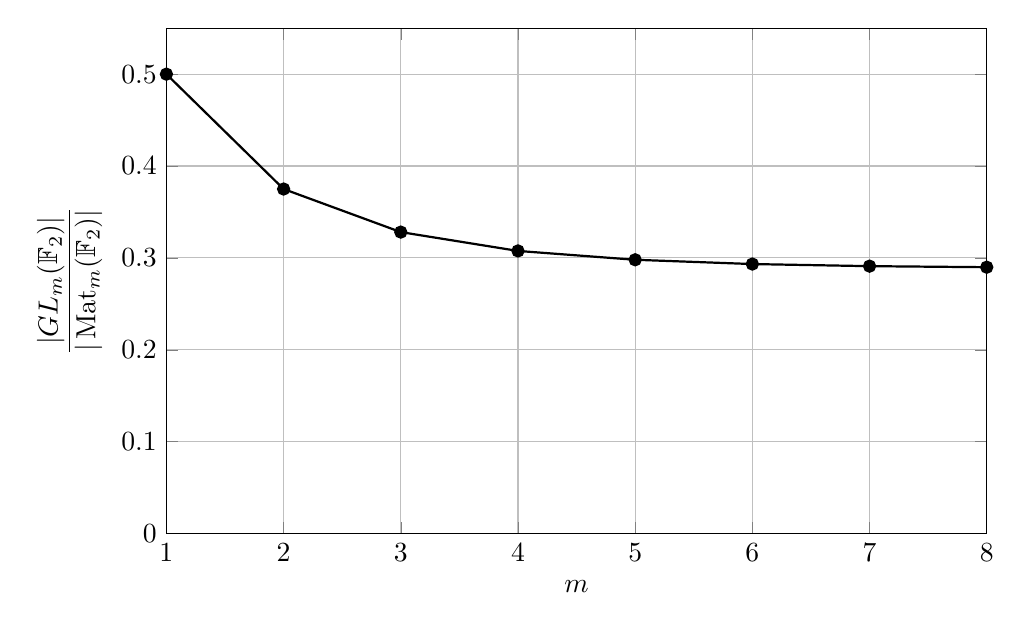
\begin{tikzpicture}
			\begin{axis}[
				width=12cm,
				height=8cm,
				xlabel={$m$},
				ylabel={$\dfrac{|GL_m(\F_2)|}{|\Mat_m(\F_2)|}$},
				ymin=0,
				ymax=0.55,
				xmin=1,
				xmax=8,
				xtick={1,2,3,4,5,6,7,8},
				ymajorgrids=true,
				xmajorgrids=true,
				enlargelimits=false
				]
				\addplot[
				mark=*,
				thick
				] coordinates {
					(1,0.5)
					(2,0.375)
					(3,0.328125)
					(4,0.3076171875)
					(5,0.298004150390625)
					(6,0.2933478355407715)
					(7,0.2910560965538025)
					(8,0.2899184823036194)
				};
			\end{axis}
		\end{tikzpicture}
	\end{center}
	
	\begin{remark}
		For fixed \(q\), the ratio
		\[
		\frac{|GL_m(\F_q)|}{|\Mat_m(\F_q)|}
		=
		\prod_{j=1}^{m}(1-q^{-j})
		\]
		decreases as \(m\) increases and converges to the infinite product
		\[
		\prod_{j=1}^{\infty}(1-q^{-j}).
		\]
		For \(q=2\), this limit is approximately \(0.288\).
	\end{remark}

\begin{center}
	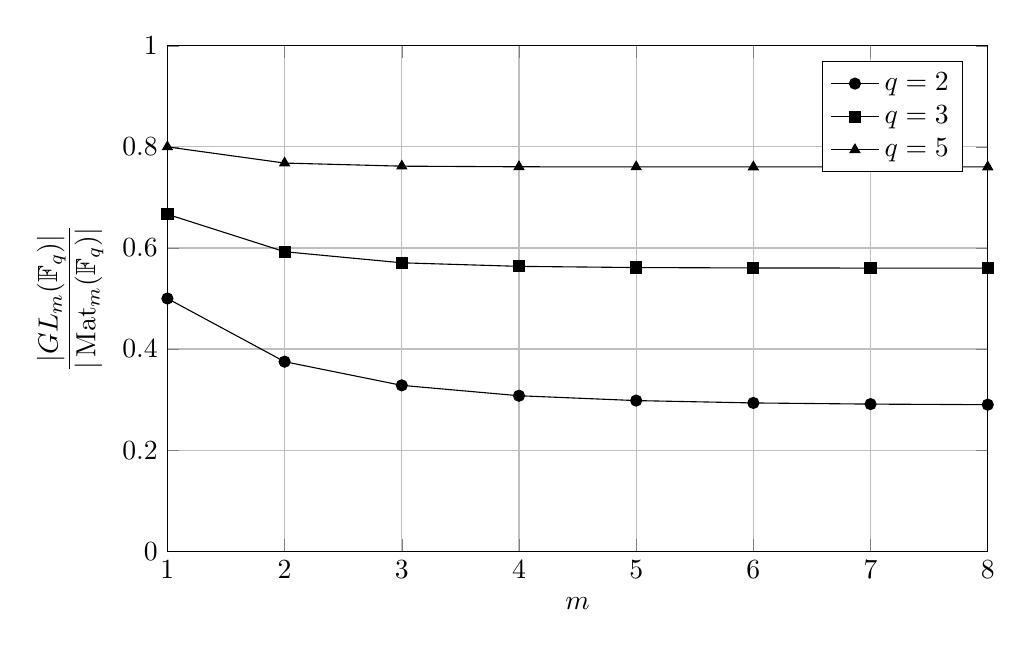
\begin{tikzpicture}
		\begin{axis}[
			width=12cm,
			height=8cm,
			xlabel={$m$},
			ylabel={$\dfrac{|GL_m(\F_q)|}{|\Mat_m(\F_q)|}$},
			ymin=0,
			ymax=1,
			xmin=1,
			xmax=8,
			xtick={1,2,3,4,5,6,7,8},
			ymajorgrids=true,
			xmajorgrids=true,
			legend style={at={(0.97,0.97)},anchor=north east}
			]
			\addplot[mark=*] coordinates {
				(1,0.5)
				(2,0.375)
				(3,0.328125)
				(4,0.3076171875)
				(5,0.298004150390625)
				(6,0.2933478355407715)
				(7,0.2910560965538025)
				(8,0.2899184823036194)
			};
			\addlegendentry{$q=2$}
			
			\addplot[mark=square*] coordinates {
				(1,0.6666666667)
				(2,0.5925925926)
				(3,0.5706447188)
				(4,0.5635989238)
				(5,0.5612511784)
				(6,0.5604553718)
				(7,0.5601834231)
				(8,0.5600901142)
			};
			\addlegendentry{$q=3$}
			
			\addplot[mark=triangle*] coordinates {
				(1,0.8)
				(2,0.768)
				(3,0.761856)
				(4,0.7606370304)
				(5,0.7603930061)
				(6,0.7603442021)
				(7,0.7603344414)
				(8,0.7603324892)
			};
			\addlegendentry{$q=5$}
		\end{axis}
	\end{tikzpicture}
\end{center}

\newpage
\begin{center}
	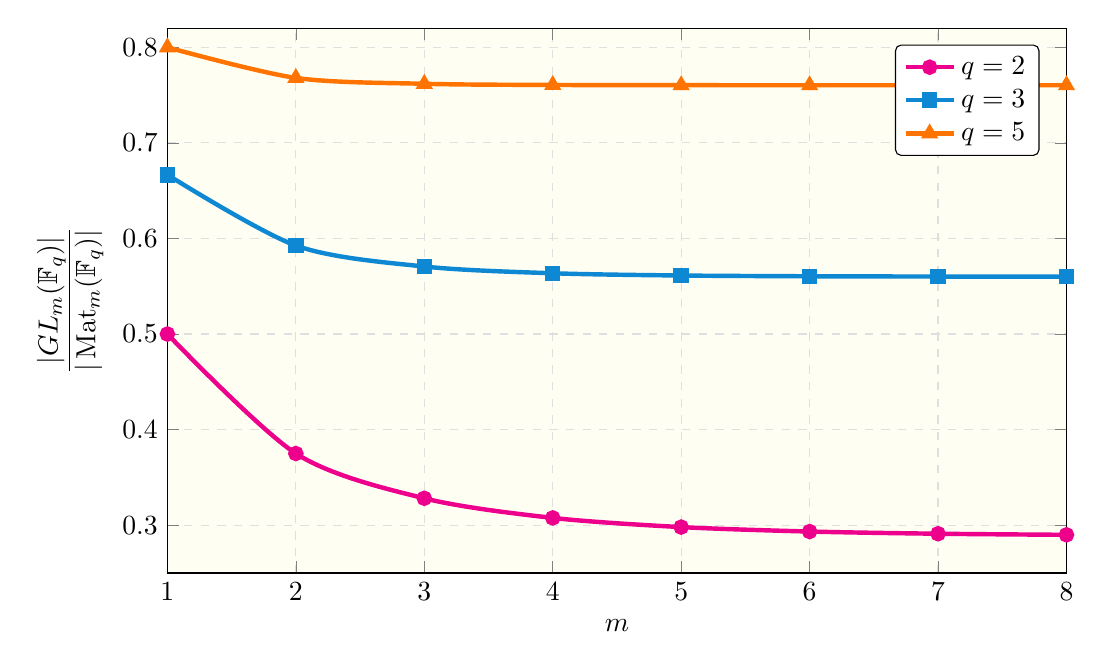
\begin{tikzpicture}
		\begin{axis}[
			width=13cm,
			height=8.5cm,
			xlabel={$m$},
			ylabel={$\dfrac{|GL_m(\F_q)|}{|\Mat_m(\F_q)|}$},
			xmin=1, xmax=8,
			ymin=0.25, ymax=0.82,
			xtick={1,2,3,4,5,6,7,8},
			ymajorgrids=true,
			xmajorgrids=true,
			grid style={dashed, gray!25},
			axis background/.style={fill=yellow!5},
			legend style={
				at={(0.97,0.97)},
				anchor=north east,
				draw=black,
				fill=white,
				rounded corners=2pt
			},
			every axis plot/.append style={ultra thick}
			]
			
			\addplot[
			color=magenta,
			mark=*,
			mark options={fill=magenta},
			smooth
			] coordinates {
				(1,0.5)
				(2,0.375)
				(3,0.328125)
				(4,0.3076171875)
				(5,0.298004150390625)
				(6,0.2933478355407715)
				(7,0.2910560965538025)
				(8,0.2899184823036194)
			};
			\addlegendentry{$q=2$}
			
			\addplot[
			color=cyan!70!blue,
			mark=square*,
			mark options={fill=cyan!70!blue},
			smooth
			] coordinates {
				(1,0.6666666667)
				(2,0.5925925926)
				(3,0.5706447188)
				(4,0.5635989238)
				(5,0.5612511784)
				(6,0.5604553718)
				(7,0.5601834231)
				(8,0.5600901142)
			};
			\addlegendentry{$q=3$}
			
			\addplot[
			color=orange!90!red,
			mark=triangle*,
			mark options={fill=orange!90!red},
			smooth
			] coordinates {
				(1,0.8)
				(2,0.768)
				(3,0.761856)
				(4,0.7606370304)
				(5,0.7603930061)
				(6,0.7603442021)
				(7,0.7603344414)
				(8,0.7603324892)
			};
			\addlegendentry{$q=5$}
			
		\end{axis}
	\end{tikzpicture}
\end{center}

\newpage
\begin{proposition}
	Let \(q\ge 2\) be fixed, and define
	\[
	a_m:=\frac{|GL_m(\F_q)|}{|\Mat_m(\F_q)|}
	=
	\prod_{j=1}^{m}(1-q^{-j}).
	\]
	Then the sequence \((a_m)_{m\ge 1}\) converges as \(m\to\infty\). Moreover, its limit is positive.
\end{proposition}

\begin{proof}
	For each \(j\ge 1\), we have
	\[
	0<1-q^{-j}<1.
	\]
	Hence
	\[
	0<a_m\le 1
	\]
	for all \(m\ge 1\).
	
	Also,
	\[
	a_{m+1}=a_m(1-q^{-(m+1)}),
	\]
	and since \(0<1-q^{-(m+1)}<1\), it follows that
	\[
	a_{m+1}<a_m.
	\]
	Thus \((a_m)\) is a decreasing sequence of positive real numbers. Therefore it converges to some limit
	\[
	L\ge 0.
	\]
	
	It remains to show that \(L>0\). Since \(q\ge 2\), we have \(0<q^{-j}\le 1/2\) for all \(j\ge 1\). Using the estimate
	\[
	\log(1-x)\ge -2x
	\qquad\text{for } 0\le x\le \tfrac12,
	\]
	we obtain
	\[
	\log(1-q^{-j})\ge -2q^{-j}.
	\]
	Therefore
	\[
	\log a_m
	=
	\sum_{j=1}^{m}\log(1-q^{-j})
	\ge
	-2\sum_{j=1}^{m} q^{-j}.
	\]
	Since the geometric series
	\[
	\sum_{j=1}^{\infty} q^{-j}
	\]
	converges, the right-hand side is bounded below independently of \(m\). Hence \((\log a_m)\) is bounded below, so \((a_m)\) is bounded away from \(0\). Therefore
	\[
	L>0.
	\]
	
	Thus
	\[
	\lim_{m\to\infty}\frac{|GL_m(\F_q)|}{|\Mat_m(\F_q)|}
	=
	\prod_{j=1}^{\infty}(1-q^{-j})
	\]
	exists and is positive.
\end{proof}

\begin{proof}
	Set
	\[
	a_m=\prod_{j=1}^{m}(1-q^{-j}).
	\]
	Since each factor satisfies \(0<1-q^{-j}<1\), we have \(a_m>0\) for all \(m\). Also,
	\[
	a_{m+1}=a_m(1-q^{-(m+1)})<a_m,
	\]
	so \((a_m)\) is decreasing. Hence \((a_m)\) is decreasing and bounded below by \(0\), therefore it converges.
\end{proof}
	
\end{document}